% -----------------------------------------------
% Template for ISMIR Papers
% 2025 version, based on previous ISMIR templates

% Requirements :
% * 6+n page length maximum
% * 10MB maximum file size
% * Copyright note must appear in the bottom left corner of first page
% * Clearer statement about citing own work in anonymized submission
% (see conference website for additional details)
% -----------------------------------------------

\documentclass{article}
\usepackage[T1]{fontenc}
\usepackage[utf8]{inputenc}
\usepackage[submission]{ismir} % Remove the "submission" option for camera-ready version
\usepackage{amsmath,cite,url}
\usepackage{graphicx}
\usepackage{color}

% Title. Please use IEEE-compliant title case when specifying the title here,
% as it has implications for the copyright notice
% ------
\title{Project Design Specifications for Sound Visualizer}

% Note: Please do NOT use \thanks or a \footnote in any of the author markup

% Single address
% To use with only one author or several with the same address
% ---------------

\author{
  Ethan Huang\\
  \texttt{ethanhuang@uvic.ca}
  \and
  Brian Pham\\
  \texttt{npham49@uvic.ca}
  \and
  Benjamin Say\\
  \texttt{benbsay@gmail.com}
}
%%-------------- i couldn't get normal author thing in template
%% ------------ to work so idk if this is how it should look for
%% ------------- multiple author works, will have to double check

%\oneauthor
%  {Anonymous Authors}
%  {Anonymous Affiliations\\\texttt{anonymous@ismir.net}}
% Two addresses
% --------------
%\twoauthors
%   {First author} {School \\ Department}
%   {Second author} {Company \\ Address}

% Three addresses
% --------------
%\threeauthors
%    {Ethan Huang} {Affiliation 1 \\ \texttt{author1@ismir.edu}}
%   {Brian Pham} {Affiliation 2 \\ \texttt{author2@ismir.edu}}
%   {Benjamin Say} {Affiliation 3 \\ \texttt{author3@ismir.edu}}

% Four or more addresses
% OR alternative format for large number of co-authors
% ------------
% \multauthor
%   {First author$^1$ \hspace{1cm} Second author$^1$ \hspace{1cm} Third author$^2$}
%   {{\bf Fourth author$^3$ \hspace{1cm} Fifth author$^2$ \hspace{1cm} Sixth author$^1$}\\
%   $^1$ Department of Computer Science, University, Country\\
%   $^2$ International Laboratories, City, Country\\
%   $^3$ Company, Address\\
%   {\tt\small CorrespondenceAuthor@ismir.edu, PossibleOtherAuthor@ismir.edu}
%   }

% For the author list in the Creative Common license, please enter author names.
% Please abbreviate the first names of authors and add 'and' between the second to last and last authors.
\def\authorname{F. Author, S. Author, and T. Author}

% Optional: To use hyperref, uncomment the following.
% \usepackage[bookmarks=false,pdfauthor={\authorname},pdfsubject={\pdfsubject},hidelinks]{hyperref}
% Mind the bookmarks=false option; bookmarks are incompatible with ismir.sty.

\sloppy % please retain sloppy command for improved formatting

\begin{document}

\maketitle

\begin{abstract}
%The abstract should be placed at the top left column and should contain about 150--200 words.sdkfljasd
This project aims to recreate popular visualization features similar to those built into classic multimedia programs. We seek to implement the visualization of different frequencies in music through the use of Python and Pygame.
\end{abstract}

\section{Introduction}\label{sec:introduction}
%This template includes all the information about formatting manuscripts for the ISMIR \conferenceyear\ Conference. Please follow these guidelines to give the final proceedings a uniform look. Most of the required formatting is achieved automatically by using the supplied style file (\LaTeX) or template (Word). If you have any questions, please contact the Program Committee (\texttt{ismir\conferenceyear-papers@ismir.net}). This template can be downloaded from the ISMIR \conferenceyear\ website (\texttt{https://ismir\conferenceyear.ismir.net}).

\subsection{Background}
During the 2000s, multimedia software such as iTunes and Windows Media Player came equipped with a functionality called visualization. Behind the scenes, the visualizer takes different frequencies over the track and generates detailed geometric sequences. Our project goal is to recreate this functionality with Python. 

\subsection{High-level summary}
On a high level, sounds are combinations of different frequencies; through the usage of Pygame's rendering capabilities, each frequency can be mapped into different objects in a 2-dimensional space, allowing for visualization. Pygame's rendering engine allows for different visual manipulation techniques such as resizing, colour switch, and masking, which can handle complex frequency changes and combinations. 

\subsection{Related works}
%maybe need background/related work? Done!

\begin{itemize}
    \item Music Visualization using frequencies \url{https://gitlab.com/avirzayev/music-visualizer}
    \item Music Visualization GUI \url{https://github.com/djfun/audio-visualizer-python/}
    
\end{itemize}


% We adopt a ``\textbf{(6+n)-page policy}'' for ISMIR \conferenceyear. That is, each paper may have a maximum of six pages of technical content (including figures and tables), with additional optional pages that contain only references and acknowledgments. \textbf{Note that acknowledgments should not be included in the anonymized submission.}

% Paper should be submitted as a PDF file. \textbf{The file size is limited to 10MB.} Please compress images and figures as necessary before submitting.

\iffalse 
TODO:
-get the 15 minimum references (cur: 14)
    -add datasets to references (thank god this helps pad our count lol)
-add more to abstract section (150 words ish?)
-fill in Ethan Huang stuff in roles
    - yea idk what to put there lmao
    
potential todo (maybe not necessary):
- how tf are we supposed to "... describe the ... associate literature that the group is going to use for the project".
    - hard to do for all 15 total references..
    - idk if this is intended to have an entire section to describe how we are going to use each paper because that would seem weird
-add more specificity and precision to roles
    -hard to think of so early in the project
    -hard to balance quantity and difficulty and order or tasks between each member
    -specific objectives for project?
\fi

\break

\section{Methodology}

% tried to format this so that it fit nicely into one column of a page, is there a chance we can keep that? -ben
% datasheets sourced from: https://labs.freesound.org/datasets/

% i think Ethan mentioned it's a template thing unfortunately - brian
\subsection{Datasets}

Four different datasets were chosen for testing. The goal of selecting multiple datasets was to introduce as much variance as possible into the testing to ensure the product will be effective on any type of sound. \newline

Environmental audio was chosen for the range of frequencies it presents, as well as its relatively low volume levels. This ensures that the product is both sensitive enough and can work on a wide enough range of frequencies. Likewise, testing with the Goodsounds dataset (solo musical instruments) will help ensure that the visuals “fit” subjectively with the perception of the musicality of the audio file. For example, the audio clips of musical instruments playing scales will be used to ensure the visualizer can move linearly if necessary. \newline

The Mixed Emotional Music Soundscape is created from an assortment of 6-second Creative Commons licensed audio clips. These clips have been used to study variance in emotional response depending on the mixing and composition of music. The Freesound loop dataset contains clips from music within a range of BPM and genre. Testing with these datasets will ensure that the visualizer can represent the perceived "tone" of the audio file. \newline

\begin{itemize}
    \item Environmental Audio: \url{https://zenodo.org/records/1069747#.Xlj0vi2ZN24}
    \item Solo Musical Instruments Dataset: \url{https://zenodo.org/records/820937#.Xlj1by2ZN24}
    \item Mixed Emotional Music Soundscape: \url{https://www.metacreation.net/projects/emo-soundscapes/}
    \begin{itemize}
        \item Research Paper: \url{https://static1.squarespace.com/static/64487a14945a646fa6f7a229/t/64f94111f82e5559e265c0cb/1715876819379/2017-Emo-Soundscapes-ADatasetforSoundscapeEmotionRecognition.pdf}
    \end{itemize}
    \item Freesound Loop Dataset: \url{https://zenodo.org/records/3967852}
    \begin{itemize}
        \item Research Paper: \url{https://program.ismir2020.net/poster_2-16.html}
    \end{itemize}
\end{itemize}


\subsection{Tools}
\begin{itemize}
    \item Python: main programming language \url{https://www.python.org/}
    \item Pygame: library for graphical processing \url{https://www.pygame.org/news}
    \item Numpy: library for data processing \url{https://librosa.org/doc/latest/index.html}
    \item Librosa: library for handling sound input and processing \url{https://librosa.org/doc/latest/index.html}
    \item GitHub: for hosting and managing source code \url{https://github.com/}
    \item Overleaf: for creating reports and summaries in LaTeX \url{https://www.overleaf.com/}
\end{itemize}


\section{Timeline, objectives and roles}

% The proceedings will be printed on \underline{portrait A4-size paper} \underline{(21.0cm x 29.7cm)}. All material on each page should fit within a rectangle of 17.2cm x 25.2cm, centered on the page, beginning 2.0cm from the top of the page and ending with 2.5cm from the bottom. The left and right margins should be 1.9cm. The text should be in two 8.2cm columns with a 0.8cm gutter. All text must be in a two-column format. Text must be fully justified.

\subsection{Timeline and objectives}
Timeline assuming the project submission date is April 4th, 2025.
\begin{enumerate}
    \item Define Minimum Viable Product (MVP) specifications using requirements and user stories and define a set of functionalities to be present in the MVP. Initial deadline: Feb 26th, 2025
    \begin{enumerate}
        \item Brian Pham: Create a series of user stories for graphical output
        \item Ethan Huang: Create a series of user stories for Graphical User Interface (GUI)
        \item Benjamin Say: Create a series of requirements for data processing
        \item Whole team: Agree on the functionalities to be developed for MVP\end{enumerate}
    \item Develop MVP with agreed-upon functionalities. Initial deadline: Mar 10th, 2025
    \begin{enumerate}
        \item Brian Pham: Develop with a focus on graphical output
        \item Ethan Huang: Develop with a focus on GUI
        \item Benjamin Say: Develop with a focus on music data processing
        \item Whole team: Combine work, resolve merge-conflicts\end{enumerate}
    \item Initial run and bug fixes. Initial deadline: Mar 17th, 2025
    \begin{enumerate}
        \item Whole team: Test run against user stories and create a log of bugs and defects
        \item Brian Pham: Fix graphical output-related bugs
        \item Ethan Huang: Fix GUI-related bugs
        \item Benjamin Say: Fix music data processing-related bugs \end{enumerate}
    \item Create a demo for TA and Prof and receive feedback on project direction. Initial deadline: Mar 19th, 2025
    \begin{enumerate}
        \item Whole team: Record demo and send to TA and prof \end{enumerate}
    \item Create final project specifications based on feedback. Initial deadline: Mar 22nd, 2025
    \begin{enumerate}
        \item Brian Pham: Create a set of specifications based on feedback for graphical output
        \item Ethan Huang: Create a set of specifications based on feedback for GUI
        \item Benjamin Say: Create a set of specifications based on feedback for music data processing \end{enumerate}
    \item Develop the final product with agreed-upon specifications. Initial deadline: Mar 31st, 2025
    \begin{enumerate}
        \item Brian Pham: Develop with a focus on graphical output
        \item Ethan Huang: Develop with a focus on GUI
        \item Benjamin Say: Develop with a focus on music data processing 
        \item Whole team: Combine work, resolve merge-conflicts\end{enumerate}
    \item Create demo, complete documentation, and submit the project. Original deadline: April 4th, 2025
    \begin{enumerate}
        \item Whole team: Create demo, final report, and submit project \end{enumerate}
\end{enumerate}


\subsection{Roles}

\begin{itemize}
    \item Brian Pham: Graphical Output Development
    \item Benjamin Say: Music Data Processing Development
    \item Ethan Huang: Graphical User Interface Development
\end{itemize}

% \section{Typeset Text}\label{sec:typeset_text}

% \subsection{Normal or Body Text}\label{subsec:body}

% Please use a 10pt (point) Times font. Sans-serif or non-proportional fonts can be used only for special purposes, such as distinguishing source code text.

% The first paragraph in each section should not be indented, but all other paragraphs should be.

% \subsection{Title and Authors}

% The title is 14pt Times, bold, caps, upper case, centered. \textbf{Authors' names are omitted when submitting for double-blind reviewing.}

% \subsection{First Page Copyright Notice}

% Please include the copyright notice exactly as it appears here in the lower left-hand corner of the page. It is set in 8pt Times.


% \subsection{Page Numbering, Headers and Footers}

% Do not include headers, footers or page numbers in your submission. These will be added when the publications are assembled.

% \subsection{Line Numbers}

% \textbf{Line numbers should be included in your submitted manuscript,} for reference during reviewing.

% \section{First Level Headings}

% First-level headings are in Times 10pt bold, centered with 1 line of space above the section head, and 1/2 space below it. For a section header immediately followed by a subsection header, the space should be merged.

% \subsection{Second Level Headings}

% Second-level headings are in Times 10pt bold, flush left, with 1 line of space above the section head, and 1/2 space below it. The first letter of each significant word is capitalized.

% \subsubsection{Third and Further Level Headings}

% Third-level headings are in Times 10pt italic, flush left, with 1/2 line of space above the section head, and 1/2 space below it. The first letter of each significant word is capitalized. Using more than three levels of headings is highly discouraged.

% \section{Footnotes and Figures}

% \subsection{Footnotes}

% Indicate footnotes with a number in the text.\footnote{This is a footnote.} Use 8pt type for footnotes. Place the footnotes at the bottom of the page on which they appear. Precede the footnote with a 0.5pt horizontal rule.

% \subsection{Figures, Tables and Captions}

% All artwork must be centered, neat, clean, and legible. All lines should be very dark for purposes of reproduction and art work should not be hand-drawn. The proceedings are not in color, and therefore all figures must make sense in black-and-white form. \textbf{Figure and table numbers and captions always appear below the figure.} Leave 1 line space between the figure or table and the caption. Each figure or table is numbered consecutively. Captions should be Times 10pt. Place tables/figures in text as close to the reference as possible. References to tables and figures should be capitalized, for example, see \figref{fig:example} and \tabref{tab:example}. Figures and tables may extend across both columns to a maximum width of 17.2cm.

% \textbf{To enhance accessibility, we strongly encourage the authors to adopt a color blind friendly color palette when making plots.} For Matplotlib users, the `tableau-colorblind10' and `petroff10' color palettes would be good options, which can be enabled by \texttt{plt.style.use('tableau-colorblind10')} and \texttt{plt.style.use('petroff10')}.

% \begin{table}
%   \centering
%   \begin{tabular}{|l|l|}
%     \hline
%     String value & Numeric value \\
%     \hline
%     Hello ISMIR  & \conferenceyear \\
%     \hline
%   \end{tabular}
%   \caption{Table captions should be placed below the table.}
%   \label{tab:example}
% \end{table}

% \begin{figure}
%   \centering
%   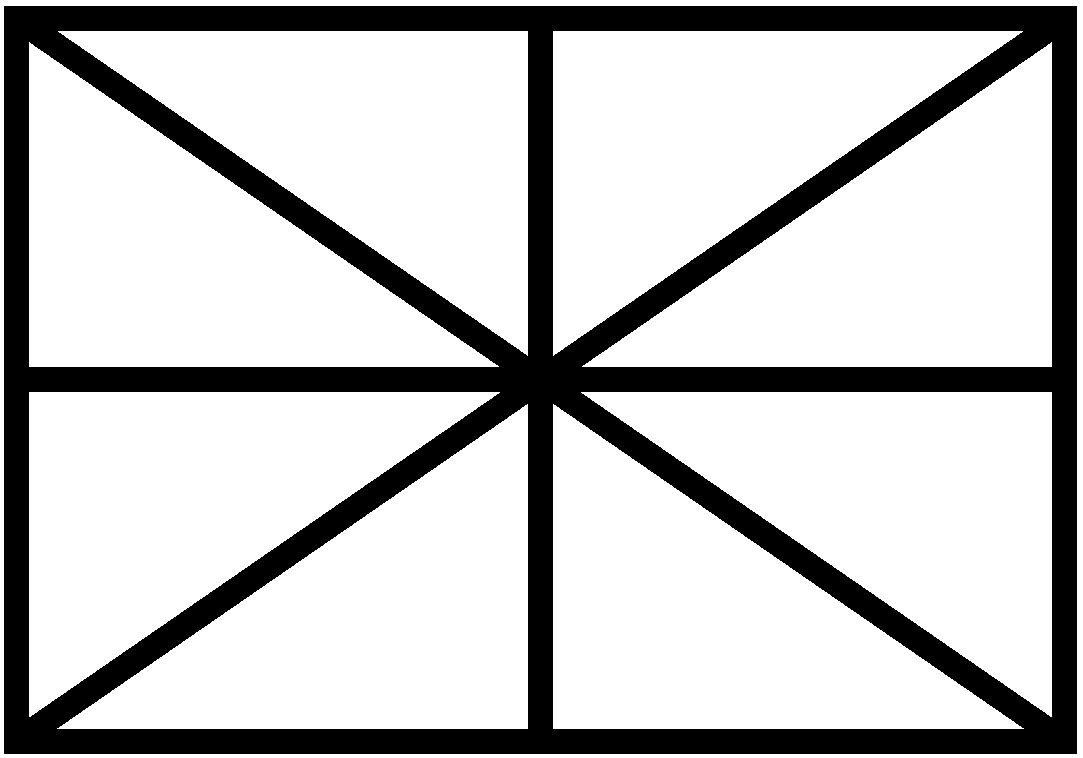
\includegraphics[alt={ISMIR 2025 template example image},width=0.9\linewidth]{example.png}
%   \caption{Figure captions should be placed below the figure.}
%   \label{fig:example}
% \end{figure}

% \section{Equations}

% Equations should be placed on separate lines and numbered. The number should be on the right side, in parentheses, as in \eqnref{relativity}.

% \begin{equation}\label{relativity}
% E=mc^{2}
% \end{equation}

% \section{Citations}

% All bibliographical references should be listed at the end of the submission, in a section named ``REFERENCES,'' numbered and in the order that they first appear in the text. Formatting in the REFERENCES section must conform to the IEEE standard (\url{https://ieeeauthorcenter.ieee.org/wp-content/uploads/IEEE-Reference-Guide.pdf}). Approved IEEE abbreviations (Proceedings $\rightarrow$ Proc.) may be used to shorten reference listings. All references listed should be cited in the text. When referring to documents, place the numbers in square brackets (e.g., \cite{ISMIR17Author:01} for a single reference, or \cite{JNMR10Someone:01,Book20Person:01,Chapter09Person:01} for a range).

% \textbf{As submission is double blind, refer to your own published work in the third person.} That is, use ``In the previous work of \cite{ISMIR17Author:01},'' not ``In our previous work \cite{ISMIR17Author:01}.'' If you cite your other papers that are not widely available (e.g., a journal paper under review), use anonymous author names in the citation, e.g., an author of the form ``A. Anonymous.''

% \section{Acknowledgments}

% You may include an optional Acknowledgments section in your camera-ready version to refer to any individuals or organizations that should be acknowledged in your paper. \textbf{Do not include the Acknowledgments section in your submitted manuscript.} The Acknowledgments section does \textit{not} count towards the page limit for scientific content.

% \section{Ethics Statement}

% You may include an optional Ethics Statement section to provide additional ethical considerations related to your paper. The Ethics Statement section can be included both at submission time and in your camera-ready version. See the Call for Papers for details. The Ethics Statement section does \textit{not} count towards the page limit for scientific content.

% \section{Camera Ready Preparation}\label{sec:cameraready}

% \textbf{The camera-ready version should include the names, affiliations and email addresses of the authors.} Authors' names are centered. The lead author's name is to be listed first (left-most), and the co-authors' names after. If the addresses for all authors are the same, include the address only once, centered. If the authors have different addresses, put the addresses, evenly spaced, under each authors' name. To display the author information in \LaTeX, please remove the global option `submission' when importing the `ismir' package (i.e., \texttt{\textbackslash usepackage\{ismir\}} in line 16).

% \textbf{Please make sure that the author names, paper title and proceedings title are shown correctly in the copyright notice.} For \LaTeX\ users, the proceedings title will be automatically loaded when you remove the global option `submission' when importing the `ismir' package (i.e., \texttt{\textbackslash usepackage\{ismir\}} in line 16). For Word users, you will need to manually replace ``submitted to \textit{ISMIR}, 2025'' to ``in \textit{Proc. of the 26th Int. Society for Music Information Retrieval Conf.}, Daejeon, South Korea, 2025.''

% \textbf{You must also remove all line numbers from the final camera-ready version.} This can be done in \LaTeX\ by removing the global option `submission' when importing the ismir package (i.e., \texttt{\textbackslash usepackage\{ismir\}} in line 16). This can be done in Microsoft Word by selecting ``Layout > Line Numbers > None.''

% % For BibTeX users:
% \bibliography{ISMIRtemplate}

% % For non BibTeX users:
\iffalse
**double check if titles of papers are right format.
i just capitalized first letter of every word but ye
\fi

\newpage
\begin{thebibliography}{citations}

%\bibitem{Author:17}
%E.~Author and B.~Authour, ``The title of the conference paper,'' in {\em Proc.
%of the Int. Society for Music Information Retrieval Conf.}, (Suzhou, China),
%pp.~111--117, 2017.

\bibitem{savelsberg}
J.~Savelsberg, ``Visualizing Music Structure Using Spotify Data,''
in {\em ISMIR}, 2021. [Online]. Available: \url{https://archives.ismir.net/ismir2021/latebreaking/000003.pdf}

\bibitem{isaacson}
E.~Isaacson, ``What You See Is What You Get: On Visualizing Music,''
in {\em ISMIR}, 2005. [Online]. Available: \url{https://ismir2005.ismir.net/proceedings/1129.pdf}

\bibitem{takashi}
T.~Takashi, S.~Fukayama, and M.~Goto, ``Instrudive: A music Visualization System Based On Automatically Recognized Instrumentation,''
in {\em ISMIR}, 2018. [Online]. Available: \url{https://archives.ismir.net/ismir2018/paper/000063.pdf}

\bibitem{paulus}
J.~Paulus, M.~M\"uller, and A.~Klapuri, ``Audio-based Music Structure Analysis,''
in {\em ISMIR}, 2010. [Online]. Available: \url{https://ismir2010.ismir.net/proceedings/ismir2010-107.pdf}

\bibitem{thottathil}
I.~A. Thottathil and S.~Thivaharan, ``Virtual Musical Instruments with Python and OpenCV,'' \emph{Journal of Ubiquitous Computing and Communication Technologies}, vol. 5, no. 1, pp. 1–20, Mar. 2023, doi: \url{https://doi.org/10.36548/jucct.2023.1.001}.

\bibitem{mcfee}
B.~McFee, C.~Raffel, D.~Liang, D.~Ellis, M.~McVicar, E.~Battenberg, and O.~Nieto, ``librosa: Audio and Music Signal Analysis in Python,'' in \emph{Proc. Python Sci. Conf.}, 2015, pp. 18–24, doi: \url{https://doi.org/10.25080/majora-7b98e3ed-003}.

\bibitem{suman}
S.~Suman, K. S.~Sahoo, C.~Das, N. Z.~Jhanjhi, and A.~Mitra, ``Visualization of Audio Files Using Librosa,'' in \emph{Proc. 2nd Int. Conf. Math. Model. Comput. Sci.}, ser. Advances in Intelligent Systems and Computing, vol. 1422. Singapore: Springer, 2022, pp. 1–10, doi: \url{https://doi.org/10.1007/978-981-19-0182-9_41}.

\bibitem{kinsley}
H.~Kinsley and W.~McGugan, ``Creating Visuals,'' in \emph{Beginning Python Games Development}. Berkeley, CA: Apress, 2015, pp. 1–20, doi: \url{https://doi.org/10.1007/978-1-4842-0970-7_4}.

\bibitem{ishibashi}
T.~Ishibashi, Y.~Nakao, and Y.~Sugano, ``Investigating Audio Data Visualization for Interactive Sound Recognition,'' in \emph{Proc. 25th Int. Conf. Intell. User Interfaces (IUI '20)}, New York, NY, USA: Association for Computing Machinery, 2020, pp. 67–77, doi: \url{https://doi.org/10.1145/3377325.3377483}.

\bibitem{lagrange}
M.~Lagrange, M.~Rossignol, and G.~Lafay, ``Visualization Of Audio Data Using Stacked Graphs,'' in \emph{ISMIR}, 2018. [Online]. Available: \url{https://zenodo.org/records/1492531}.

\bibitem{eklund}
V.-V.~Eklund, ``DBR Dataset,'' Zenodo, Dec. 03, 2017. [Online]. Available: \url{https://doi.org/10.5281/zenodo.1069747}.

\bibitem{picas}
O.~Romani Picas, H.~Parra Rodriguez, D.~Dabiri, and X.~Serra, ``Good-sounds Dataset,'' Zenodo, Jun. 29, 2017. [Online]. Available: \url{https://doi.org/10.5281/zenodo.820937}.

\bibitem{fan}
J.~Fan, M.~Thorogood, and P.~Pasquier, ``Emo-Soundscapes: A Dataset for Soundscape Emotion Recognition,'' in \emph{Proc. Int. Conf. Affective Comput. Intell. Interaction (ACII)}, 2017.

\bibitem{ramires}
A.~Ramiresm, ``Freesound Loop Dataset,'' Zenodo, Jul. 30, 2020. [Online]. Available:\url{https://doi.org/10.5281/zenodo.3967852}

\bibitem{knees}
P.~Knees, M.~Schedl, and M.~Goto, ``Intelligent User Interfaces for music Discovery: the past 20 years and what’s to come.'' in \emph{ISMIR}, 2019. [Online]. Available: \url{http://archives.ismir.net/ismir2019/paper/000003.pdf}


% \bibitem{Person:20}
% O.~Person, {\em Title of the Book}.
% \newblock Montr\'{e}al, Canada: McGill-Queen's University Press, 2021.

% \bibitem{Person:09}
% F.~Person and S.~Person, ``Title of a chapter this book,'' in {\em A Book
% Containing Delightful Chapters} (A.~G. Editor, ed.), pp.~58--102, Tokyo,
% Japan: The Publisher, 2009.

\end{thebibliography}

\end{document}
